\section{Decodificación de códigos compactos Sprott}

Este capítulo desarrolla con todos los pasos intermedios el contrato matemático y
algorítmico que usa el Explorador Sprott. La cadena visible en la interfaz es una
representación compacta de una familia
de ecuaciones y de sus coeficientes. El recorrido completo es
\[
\begin{aligned}
\text{texto de entrada}
&\longrightarrow \text{normalización}
\longrightarrow \text{familia}
\longrightarrow \text{coeficientes}\\
&\longrightarrow \text{base de monomios}
\longrightarrow \text{matriz}
\longrightarrow \text{mapa o flujo}\\
&\longrightarrow \text{simulación}
\longrightarrow \text{descarte transitorio}
\longrightarrow \text{filtros}\\
&\longrightarrow \text{estimación rápida}
\longrightarrow \text{representación}
\longrightarrow \text{registro reproducible}.
\end{aligned}
\]
Cada flecha corresponde a una decisión concreta del programa. Conocerla permite
distinguir el sistema matemático, la aproximación numérica, el diagnóstico heurístico
y el estilo de la figura.\footnote{Lectura complementaria: J. C. Sprott,
\emph{Strange Attractors: Creating Patterns in Chaos} (1993), cap.~2,
\emph{Wiggly Lines}, en especial 2.4 \emph{The Computer Search}, y cap.~3,
\emph{Pieces of Planes}.}

\begin{idea}{Alfabetos de familia y sistemas clásicos}
Las letras de familia \codigo{A}--\codigo{X} del código compacto clasifican mapas y
flujos polinomiales por dimensión y grado. Los nombres clásicos \emph{Sprott A},
\emph{Sprott B}, \ldots, \emph{Sprott S} designan diecinueve flujos tridimensionales
específicos de la literatura. Por ejemplo, una cadena que comienza con \codigo{Q}
pertenece a la familia de \emph{flujos polinomiales 3D cuadráticos}. El sistema clásico
Sprott Q se identifica mediante su ecuación y coeficientes propios. Esta distinción se mantendrá en todas las
tablas y actividades.
\end{idea}

\subsection{Secuencia de decodificación del código}

\begin{enumerate}[label=\arabic*.]
 \item Normalizar la cadena: mayúsculas y eliminación de espacios, guiones y
       subrayados.
 \item Usar el primer carácter para consultar la familia, dimensión, grado, tipo
       y número esperado de coeficientes.
 \item Decodificar los caracteres restantes con \(c=(\operatorname{ord}-77)/10\)
       y conservar las advertencias.
 \item Si la familia es polinomial, construir la base ordenada de monomios,
       completar con ceros o truncar si la longitud no coincide, y acomodar los
       coeficientes por filas en \(C\). Si es especial, instanciar su regla
       explícita; \codigo{Z} se detiene como pendiente.
 \item Fijar \(\mathbf{x}_0=(0.1,\ldots,0.1)\).
 \item Para un mapa, iterar \(F\). Para un flujo, aproximar
       \(\dot{\mathbf{x}}=F(\mathbf{x})\) con el método y \(h\) elegidos. El
       backend C se intenta en las familias polinomiales y Python actúa como
       respaldo; las especiales usan Python.
 \item Detectar valores no finitos o cruce del umbral durante la simulación y
       conservar el estado de terminación disponible.
 \item Descartar por índice las primeras \(N_{\mathrm{tr}}\) muestras.
 \item Aplicar a la cola los filtros de divergencia, punto fijo, tamaño mínimo,
       dispersión y repetición redondeada, en ese orden.
 \item En la tabla de búsqueda, si sobrevive como
       \codigo{candidate\_chaotic}, calcular el Lyapunov rápido de 350 pasos
       mediante dos trayectorias.
 \item Eliminar filas no finitas para la representación, submuestrear si hace
       falta, proyectar, calcular la variable de color y, si se pidió, cuantizarla
       en bandas.
 \item Exportar por separado imagen, metadatos y trayectoria; completar
       manualmente los datos de procedencia que el exportador omite.
\end{enumerate}

\subsection{Normalización y selección de familia}

El analizador convierte el texto a mayúsculas y elimina espacios, guiones y
subrayados. Así, una escritura con separadores visuales se reduce a una sola cadena.
El primer carácter de la cadena limpia selecciona la familia. Los caracteres
posteriores se leen como coeficientes. Conviene conservar siempre el código original
en el informe, porque la normalización puede hacer que dos escrituras distintas
produzcan la misma cadena interna.

Cuando el primer carácter queda fuera de la tabla implementada, la familia recibe el estado
\codigo{unknown}. Una familia reconocida con semántica numérica pendiente puede decodificarse como registro de lectura; \codigo{Z} ilustra ese estado actual. Una
advertencia de longitud exige comprobar la transcripción original: rellenar un
coeficiente ausente con cero produce un sistema bien definido y fija una definición distinta de la fuente que se pretendía copiar.

\subsection{Conversión de caracteres en coeficientes}

Para cada carácter de coeficiente \(\chi\), el Explorador aplica
\[
 c(\chi)=\frac{\operatorname{ord}(\chi)-77}{10}.
\]
Por tanto, \codigo{M} representa cero y cada posición alfabética cambia el valor en
una décima. La tabla siguiente contiene el alfabeto \codigo{A}--\codigo{Z}. El
decodificador interno admite otros caracteres ASCII imprimibles, pero para escritura
pedagógica y generación sintética conviene usar este alfabeto explícito.

\begin{longtable}{>{\ttfamily}c r >{\ttfamily}c r}
\caption{Correspondencia alfabética de coeficientes.}\\
\toprule
\multicolumn{1}{c}{Carácter} & \multicolumn{1}{c}{Valor} &
\multicolumn{1}{c}{Carácter} & \multicolumn{1}{c}{Valor}\\
\midrule
\endfirsthead
\toprule
\multicolumn{1}{c}{Carácter} & \multicolumn{1}{c}{Valor} &
\multicolumn{1}{c}{Carácter} & \multicolumn{1}{c}{Valor}\\
\midrule
\endhead
A & \(-1.2\) & N & \(0.1\)\\
B & \(-1.1\) & O & \(0.2\)\\
C & \(-1.0\) & P & \(0.3\)\\
D & \(-0.9\) & Q & \(0.4\)\\
E & \(-0.8\) & R & \(0.5\)\\
F & \(-0.7\) & S & \(0.6\)\\
G & \(-0.6\) & T & \(0.7\)\\
H & \(-0.5\) & U & \(0.8\)\\
I & \(-0.4\) & V & \(0.9\)\\
J & \(-0.3\) & W & \(1.0\)\\
K & \(-0.2\) & X & \(1.1\)\\
L & \(-0.1\) & Y & \(1.2\)\\
M & \(0.0\) & Z & \(1.3\)\\
\bottomrule
\end{longtable}

La rutina de generación aleatoria no utiliza todo ese intervalo. Para cada
coeficiente sortea uno de los diecisiete valores
\[
 \{-0.8,-0.7,\ldots,0.7,0.8\},
\]
que corresponden a \codigo{E}--\codigo{U}. La semilla reinicializa el generador:
el botón \boton{Generar codigo} produce el mismo código cada vez que se pulsa con la
misma configuración y semilla; durante \boton{Buscar candidato}, una sola
inicialización genera una secuencia reproducible de intentos.

\section{Base polinomial, conteo y matriz de coeficientes}

\subsection{Número de monomios \texorpdfstring{\(\binom{D+O}{O}\)}{C(D+O,O)}
monomios}

Sea \(\mathbf{x}=(x_1,\ldots,x_D)\) y sea \(O\) el grado máximo. Un monomio
multivariado tiene la forma
\[
 \mathbf{x}^{\boldsymbol{\alpha}}
 =x_1^{\alpha_1}\cdots x_D^{\alpha_D},
 \qquad
 \alpha_i\in\mathbb{N}_0,
 \qquad
 |\boldsymbol{\alpha}|=\sum_{i=1}^{D}\alpha_i\leq O .
\]
Para contar esos monomios se introduce una variable de holgura
\(\alpha_{D+1}=O-\sum_{i=1}^{D}\alpha_i\). Entonces
\[
 \alpha_1+\cdots+\alpha_D+\alpha_{D+1}=O
\]
es una distribución de \(O\) unidades entre \(D+1\) casillas. El argumento de
estrellas y barras da
\[
 N_{\mathrm{mon}}(D,O)=\binom{D+O}{O}.
\]
Equivalentemente, hay \(\binom{D+r-1}{r}\) monomios de grado exactamente \(r\);
la identidad del palo de hockey produce
\[
 \sum_{r=0}^{O}\binom{D+r-1}{r}=\binom{D+O}{O}.
\]
Como cada una de las \(D\) ecuaciones tiene un coeficiente por monomio, el número
total de coeficientes es
\[
 N_c(D,O)=D\binom{D+O}{O},
 \qquad
 L_{\text{código}}=1+N_c(D,O).
\]
El uno adicional corresponde a la letra de familia.\footnote{Lectura
complementaria: Sprott, \emph{Strange Attractors} (1993), cap.~3,
\emph{Pieces of Planes}, en particular 3.1 \emph{A Quadratic Map in Two
Dimensions}, y apéndice E, \emph{Summary of Equations}.}

\subsection{Orden exacto de los monomios}

El orden fija qué carácter multiplica a qué término. Primero se
agrupan los monomios por grado total \(r=0,1,\ldots,O\). Dentro de cada grado, el
exponente de \(x_1\) recorre los valores posibles en orden descendente; para cada
valor se repite recursivamente la regla con \(x_2\), y así sucesivamente. Los casos
de uso más frecuentes son
\[
\begin{aligned}
(D,O)=(1,2):\quad&
 1,\ x,\ x^2,\\
(D,O)=(2,2):\quad&
 1,\ x,\ y,\ x^2,\ xy,\ y^2,\\
(D,O)=(3,2):\quad&
 1,\ x,\ y,\ z,\ x^2,\ xy,\ xz,\ y^2,\ yz,\ z^2,\\
(D,O)=(4,2):\quad&
 1,\ x,\ y,\ z,\ w,\ x^2,\ xy,\ xz,\ xw,\ y^2,\ yz,\ yw,\ z^2,\ zw,\ w^2 .
\end{aligned}
\]
Para grados superiores se conserva la misma regla. Por ejemplo, en dos variables,
el bloque cúbico es \(x^3,x^2y,xy^2,y^3\). Esta convención debe anotarse al
intercambiar códigos con programas que usan orden lexicográfico o grevlex.

\subsection{Matriz de coeficientes del sistema}

Definamos el vector de base
\[
 \boldsymbol{\phi}_{D,O}(\mathbf{x})
 =\bigl(\mathbf{x}^{\boldsymbol{\alpha}^{(1)}},\ldots,
        \mathbf{x}^{\boldsymbol{\alpha}^{(N_{\mathrm{mon}})}}\bigr)^{\mathsf T}.
\]
Los caracteres se decodifican de izquierda a derecha y se acomodan por filas en
\[
 C=
 \begin{pmatrix}
 c_{11}&\cdots&c_{1N_{\mathrm{mon}}}\\
 \vdots&&\vdots\\
 c_{D1}&\cdots&c_{DN_{\mathrm{mon}}}
 \end{pmatrix}.
\]
El campo o mapa polinomial es, en ambos casos,
\[
 F(\mathbf{x})=C\,\boldsymbol{\phi}_{D,O}(\mathbf{x}).
\]
Lo que cambia es la interpretación: para un mapa,
\(\mathbf{x}_{n+1}=F(\mathbf{x}_n)\); para un flujo,
\(\dot{\mathbf{x}}=F(\mathbf{x})\). Una cadena de longitud incorrecta recibe una
advertencia en el analizador. En las familias polinomiales, los coeficientes
faltantes se completan con cero y los sobrantes se ignoran al formar \(C\); por
reproducibilidad, conviene registrar una tolerancia explícita.

\begin{longtable}{c l c c r r}
\caption{Familias polinomiales A--X. \(D\): dimensión; \(O\): grado;
\(N_c\): coeficientes; \(L\): longitud total de la cadena.}\\
\toprule
Familia & Interpretación & \(D\) & \(O\) & \(N_c\) & \(L\)\\
\midrule
\endfirsthead
\toprule
Familia & Interpretación & \(D\) & \(O\) & \(N_c\) & \(L\)\\
\midrule
\endhead
\codigo{A} & mapa 1D & 1 & 2 & 3 & 4\\
\codigo{B} & mapa 1D & 1 & 3 & 4 & 5\\
\codigo{C} & mapa 1D & 1 & 4 & 5 & 6\\
\codigo{D} & mapa 1D & 1 & 5 & 6 & 7\\
\codigo{E} & mapa 2D & 2 & 2 & 12 & 13\\
\codigo{F} & mapa 2D & 2 & 3 & 20 & 21\\
\codigo{G} & mapa 2D & 2 & 4 & 30 & 31\\
\codigo{H} & mapa 2D & 2 & 5 & 42 & 43\\
\codigo{I} & mapa 3D & 3 & 2 & 30 & 31\\
\codigo{J} & mapa 3D & 3 & 3 & 60 & 61\\
\codigo{K} & mapa 3D & 3 & 4 & 105 & 106\\
\codigo{L} & mapa 3D & 3 & 5 & 168 & 169\\
\codigo{M} & mapa 4D & 4 & 2 & 60 & 61\\
\codigo{N} & mapa 4D & 4 & 3 & 140 & 141\\
\codigo{O} & mapa 4D & 4 & 4 & 280 & 281\\
\codigo{P} & mapa 4D & 4 & 5 & 504 & 505\\
\codigo{Q} & flujo 3D & 3 & 2 & 30 & 31\\
\codigo{R} & flujo 3D & 3 & 3 & 60 & 61\\
\codigo{S} & flujo 3D & 3 & 4 & 105 & 106\\
\codigo{T} & flujo 3D & 3 & 5 & 168 & 169\\
\codigo{U} & flujo 4D & 4 & 2 & 60 & 61\\
\codigo{V} & flujo 4D & 4 & 3 & 140 & 141\\
\codigo{W} & flujo 4D & 4 & 4 & 280 & 281\\
\codigo{X} & flujo 4D & 4 & 5 & 504 & 505\\
\bottomrule
\end{longtable}

\begin{laboratorio}{Decodificación manual del ejemplo tipo Hénon}
Use el código \codigolargo{EWMWAMMMPMMMM}. La letra \codigo{E} indica un mapa
cuadrático 2D y los doce caracteres restantes forman dos filas de seis:
\[
 C=
 \begin{pmatrix}
 1&0&1&-1.2&0&0\\
 0&0.3&0&0&0&0
 \end{pmatrix}.
\]
Con \(\boldsymbol{\phi}_{2,2}=(1,x,y,x^2,xy,y^2)^{\mathsf T}\), resulta
\[
 x_{n+1}=1+y_n-1.2x_n^2,\qquad y_{n+1}=0.3x_n.
\]
Fije \(\mathbf{x}_0=(0.1,0.1)\), \(N=28000\), descarte \(1200\) iteraciones y
use umbral de divergencia \(10^9\). Grafique \(x_n\) contra \(y_n\). El dibujo y
los diagnósticos son evidencia numérica para esa configuración, no una prueba
global de caos.
\end{laboratorio}

\begin{figure}[H]
\centering
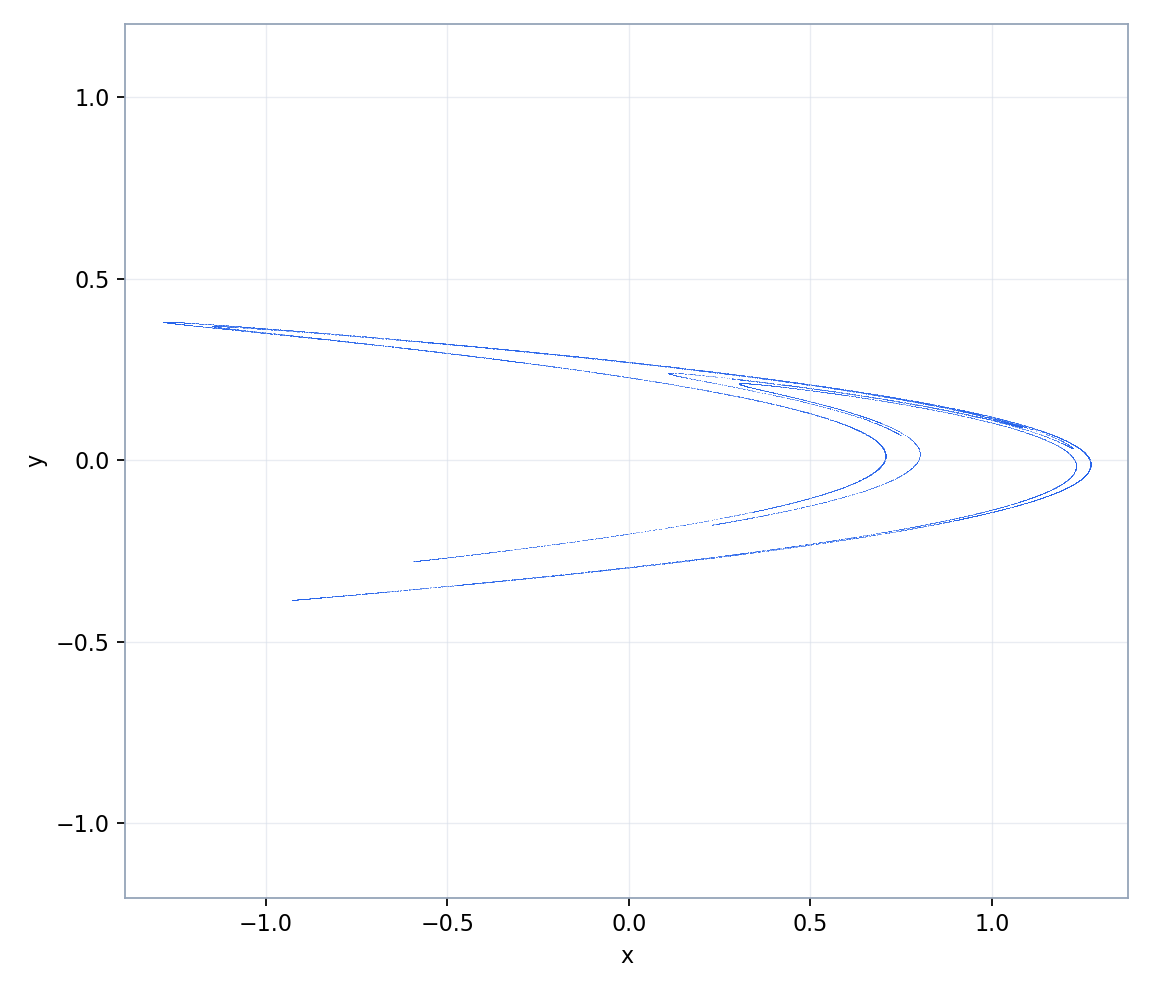
\includegraphics[width=0.73\textwidth,height=0.32\textheight,keepaspectratio]{../sprott/images/henon_like_synthetic_sprott_theory.png}
\caption{Referencia visual de un mapa tipo Hénon generada con el mismo software.
Cada punto de la nube es la imagen del anterior. Observe el
plegamiento de las ramas y compárelo con el caso decodificado, cuyos coeficientes
pueden cambiar la apertura, el espesor y la región visitada.}
\label{fig:sprott-decodificacion-henon}
\end{figure}

\section{Mapa, flujo e integración numérica}

\subsection{Actualización de mapas e integración de flujos}

En un mapa, una evaluación de \(F\) es ya un paso completo:
\[
 \mathbf{x}_{n+1}=F(\mathbf{x}_n).
\]
No intervienen \(h\), Euler ni Runge--Kutta. En un flujo, en cambio,
\[
 \frac{d\mathbf{x}}{dt}=F(\mathbf{x}),\qquad
 \mathbf{x}(0)=\mathbf{x}_0,
\]
y el programa aproxima la solución en \(t_n=nh\). Cambiar \(h\) o el integrador
no cambia la ecuación diferencial, pero sí cambia la trayectoria discreta que se
usa para diagnosticarla y dibujarla.

La condición inicial de la interfaz es fija:
\[
 \mathbf{x}_0=(0.1,\ldots,0.1).
\]
Por ello, una repetición manual debe registrar al menos código, número de pasos,
transitorio, umbral de divergencia y, para flujos, \(h\) y método. En el motor
polinomial de Python, solicitar \(N\) pasos produce \(N+1\) estados al incluir
\(\mathbf{x}_0\); las familias especiales producen \(N\) estados porque ejecutan
las actualizaciones \(n=1,\ldots,N-1\). Esta diferencia de conteo importa al
comparar exportaciones línea por línea.

\subsection{Selección del motor numérico}

La interfaz solicita primero el backend nativo C para familias polinomiales. En
mapas pasa un paso interno \(h=1\); en flujos transmite el \(h\) elegido y la clave
de Euler, Heun o RK4. Si el motor nativo produce un error de disponibilidad o de
interfaz, la ejecución vuelve al algoritmo Python. Ambos reservan \(N+1\) estados
para \(N\) pasos polinomiales, junto con un vector temporal o de índices. Las
familias especiales no entran al backend C y se calculan con su simulador Python.
El resultado interno conserva \codigo{backend} y \codigo{native\_status}, pero,
como se explica al final, el exportador JSON ordinario todavía no los incorpora.

\subsection{Euler explícito}

Integrando exactamente en \([t_n,t_n+h]\),
\[
 \mathbf{x}(t_n+h)=\mathbf{x}(t_n)+
 \int_{t_n}^{t_n+h}F(\mathbf{x}(s))\,ds.
\]
Euler aproxima el integrando por su valor izquierdo:
\[
 \boxed{\mathbf{x}_{n+1}=\mathbf{x}_n+hF(\mathbf{x}_n)}.
\]
Su error local es \(O(h^2)\) y su error global es \(O(h)\). Es barato, pero un
\(h\) grande puede fabricar inestabilidad, borrar detalles o producir divergencia
numérica incluso si la órbita continua de interés permanece acotada.

\subsection{Heun o trapecio explícito}

Heun predice primero con Euler y promedia las pendientes de los dos extremos:
\[
\begin{aligned}
 \mathbf{k}_1&=F(\mathbf{x}_n),\\
 \widetilde{\mathbf{x}}&=\mathbf{x}_n+h\mathbf{k}_1,\\
 \mathbf{k}_2&=F(\widetilde{\mathbf{x}}),\\
 \boxed{\mathbf{x}_{n+1}}&=
 \mathbf{x}_n+\frac{h}{2}(\mathbf{k}_1+\mathbf{k}_2).
\end{aligned}
\]
Tiene error local \(O(h^3)\) y global \(O(h^2)\). El motor admite este método,
aunque la selección ordinaria de la interfaz expone actualmente Euler y RK4. Para
usar Heun en un experimento automatizado hay que invocar el motor y registrarlo
explícitamente; cada figura se interpreta con la opción que declara su cálculo.

\subsection{Runge--Kutta clásico de cuarto orden}

RK4 muestrea cuatro pendientes:
\[
\begin{aligned}
 \mathbf{k}_1&=F(\mathbf{x}_n),\\
 \mathbf{k}_2&=F\!\left(\mathbf{x}_n+\frac{h}{2}\mathbf{k}_1\right),\\
 \mathbf{k}_3&=F\!\left(\mathbf{x}_n+\frac{h}{2}\mathbf{k}_2\right),\\
 \mathbf{k}_4&=F(\mathbf{x}_n+h\mathbf{k}_3),\\
 \boxed{\mathbf{x}_{n+1}}&=\mathbf{x}_n+
 \frac{h}{6}\left(\mathbf{k}_1+2\mathbf{k}_2+2\mathbf{k}_3+\mathbf{k}_4\right).
\end{aligned}
\]
Su error local es \(O(h^5)\) y el global es \(O(h^4)\) bajo las hipótesis usuales
de regularidad. El orden alto requiere comprobación de exactitud mediante repetición
con \(h/2\), comparar rangos, proyecciones y diagnósticos, y ampliar el horizonte
físico cuando sea necesario. Con \(N\) pasos, el horizonte de un flujo es
aproximadamente \(T=Nh\); duplicar \(N\) sin cambiar \(h\) extiende el tiempo,
mientras reducir \(h\) con \(N\) fijo acorta el horizonte.\footnote{Lectura
complementaria: Sprott, \emph{Strange Attractors} (1993), cap.~6,
\emph{Fields and Flows}, especialmente 6.3 \emph{Finite Differences};
J. C. Sprott, \emph{Elegant Chaos: Algebraically Simple Chaotic Flows} (2010),
cap.~1, \emph{Fundamentals}.}

\begin{idea}{Prueba práctica de convergencia}
Para un flujo, compare RK4 con \(h\), \(h/2\) y \(h/4\) manteniendo el mismo
horizonte \(T\), por lo que \(N\) debe duplicarse cada vez. Las dos
trayectorias caóticas coincidan punto a punto durante mucho tiempo. Sí se espera
consistencia cualitativa y estadística en proyecciones, rangos y diagnósticos
después de un transitorio comparable en tiempo físico.
\end{idea}

\begin{figure}[H]
\centering
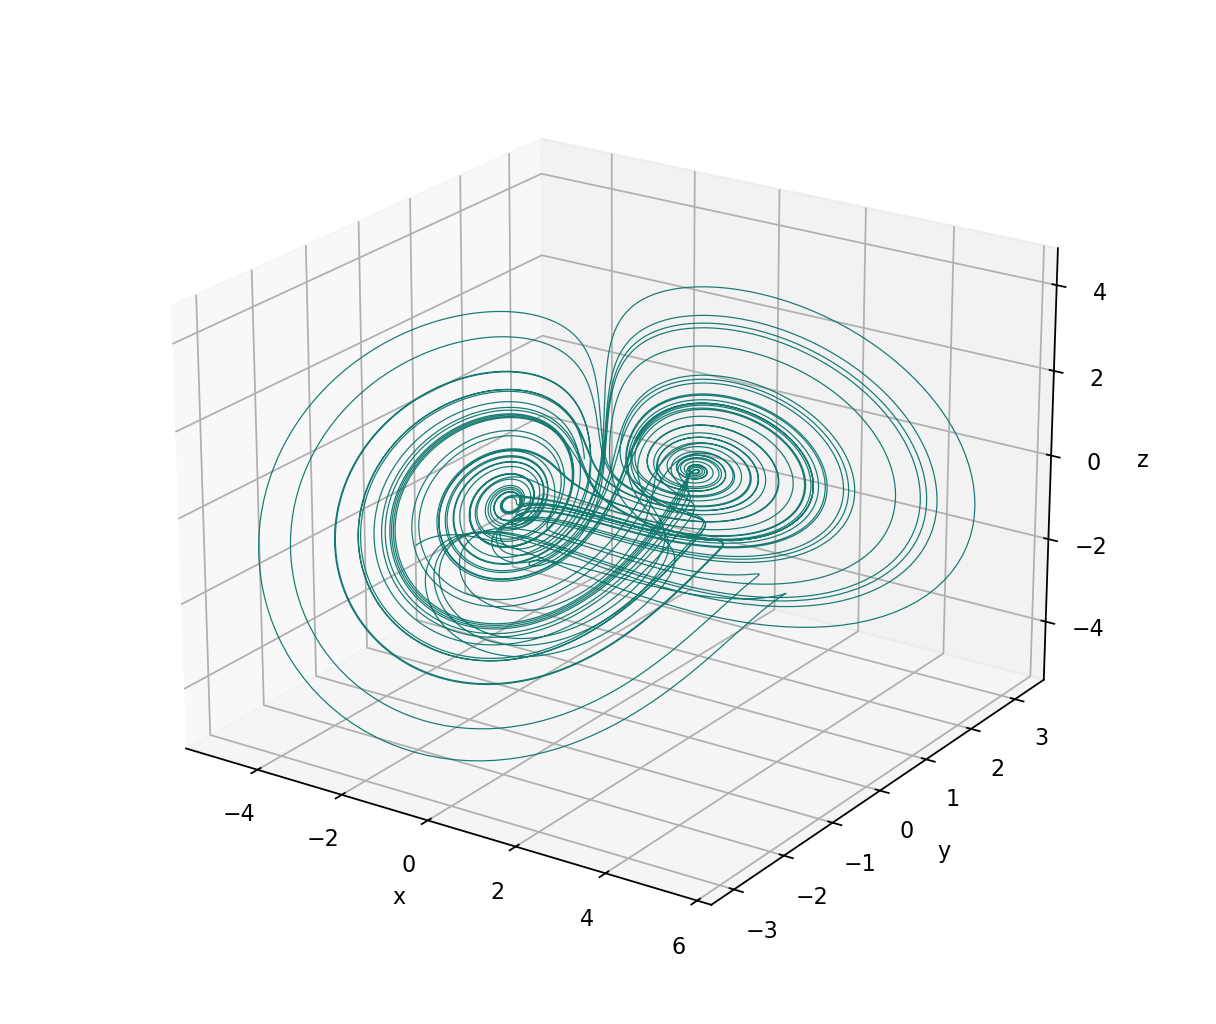
\includegraphics[width=0.74\textwidth,height=0.34\textheight,keepaspectratio]{../sprott/images/sprott_five_term_flow_theory.png}
\caption{Flujo tridimensional de cinco términos integrado con RK4. A diferencia de
la nube de un mapa, aquí las muestras consecutivas aproximan una curva continua.
Observe los giros alrededor de dos regiones y los cruces aparentes que sólo una vista
tridimensional permite separar.}
\label{fig:sprott-flujo-cinco-terminos}
\end{figure}

\begin{figure}[H]
\centering
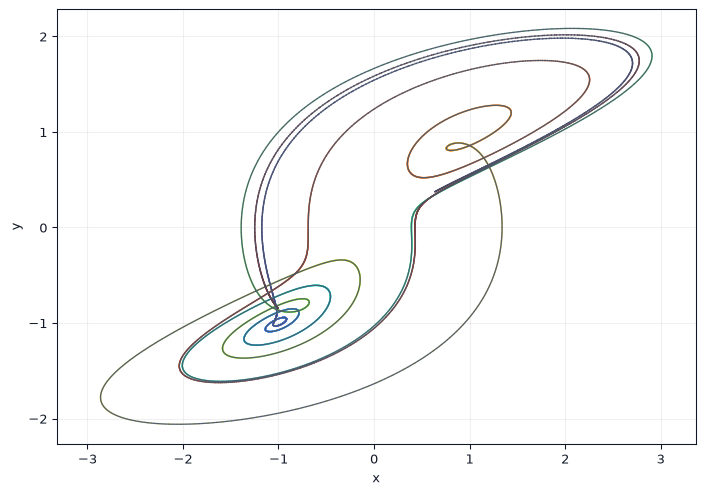
\includegraphics[width=0.72\textwidth,height=0.31\textheight,keepaspectratio]{../sprott/examples/thumbnails/synthetic_q_five_term_euler_compare.png}
\caption{Proyección \(x\)-\(y\) del mismo flujo calculada con Euler y fondo blanco.
La figura sirve como control numérico: observe la geometría gruesa y repita con RK4,
\(h/2\) y el mismo horizonte físico antes de atribuir a la ecuación una diferencia
que pudiera proceder del integrador.}
\label{fig:sprott-euler-control}
\end{figure}

\section{Familias especiales Y, Z y signos}

En esta sección \(x^+\) significa el siguiente valor de un mapa, no una derivada.
Las seis entradas especiales, incluida la clave barra inversa
(\texttt{\textbackslash}), se decodifican como familias 4D. En cinco de ellas,
\(z\) y \(w\) son variables auxiliares de visualización: \(z^+=(x^+)^2+(y^+)^2\)
y
\[
 w^+=
 \begin{cases}
 (n-1000)/(N_{\max}-1000),&N_{\max}>1000,\\
 0,&N_{\max}\leq1000.
 \end{cases}
\]
El valor de \(w\) puede ser negativo durante los primeros mil pasos; representa un
indicador de progreso y se distingue del tiempo
físico ni una cuarta ecuación autónoma.

{\footnotesize
\setlength{\tabcolsep}{3pt}
\begin{longtable}{c c p{0.59\linewidth} p{0.16\linewidth}}
\caption{Familias especiales: longitud, ecuaciones y estado de implementación.}\\
\toprule
Clave & \(L\) & Ecuaciones principales & Estado actual\\
\midrule
\endfirsthead
\toprule
Clave & \(L\) & Ecuaciones principales & Estado actual\\
\midrule
\endhead
\codigo{Y} & 11 &
\(\begin{aligned}
x^+&=a_0+a_1x+a_2y+a_3|x|+a_4|y|,\\
y^+&=a_5+a_6x+a_7y+a_8|x|+a_9|y|
\end{aligned}\);
\(z^+=(x^+)^2+(y^+)^2\), \(w^+\) como arriba. &
Implementada; 10 coeficientes.\\[2mm]
\codigo{Z} & 11 &
Está etiquetada como familia lógica AND/OR, pero no hay ecuaciones numéricas
asociadas en el registro actual. &
Reconocida con 10 coeficientes, pero semántica pendiente; no simulable.\\[2mm]
\codigo{[} & 15 &
\(\begin{aligned}
x^+={}&a_0+a_1x+a_2y+a_3|x|^{a_4}+a_5|y|^{a_6},\\
y^+={}&a_7+a_8x+a_9y+a_{10}|x|^{a_{11}}+a_{12}|y|^{a_{13}}
\end{aligned}\);
\(z^+=(x^+)^2+(y^+)^2\), \(w^+\) como arriba. &
Implementada; 14 coeficientes. Potencias negativas en base cero divergen.\\[2mm]
\texttt{\textbackslash} & 19 &
\(\begin{aligned}
x^+={}&a_0+a_1x+a_2y+a_3\sin(a_4x+a_5)+a_6\sin(a_7y+a_8),\\
y^+={}&a_9+a_{10}x+a_{11}y+a_{12}\sin(a_{13}x+a_{14})
       +a_{15}\sin(a_{16}y+a_{17})
\end{aligned}\);
\(z^+=(x^+)^2+(y^+)^2\), \(w^+\) como arriba. &
Implementada; 18 coeficientes.\\[2mm]
\codigo{]} & 7 &
\(\theta=2\pi/(13+10a_5)\), \(q=x+a_1\sin(a_2y+a_3)\);
\(\begin{aligned}
x^+&=10a_0+q\cos\theta+y\sin\theta,\\
y^+&=10a_4-q\sin\theta+y\cos\theta
\end{aligned}\);
\(z^+=(x^+)^2+(y^+)^2\), \(w^+\) como arriba. &
Implementada; 6 coeficientes. Si \(|13+10a_5|<10^{-9}\), usa
\(\theta=0\) y emite advertencia.\\[2mm]
\codigo{\textasciicircum} & 10 &
\(\begin{aligned}
x^+={}&x+0.1a_0y,\\
y^+={}&y+0.1(a_1x+a_2x^3+a_3x^2y+a_4xy^2+a_5y+a_6y^3+a_7\sin z),\\
z^+={}&\bigl[z+0.1(a_8+1.3)\bigr]\bmod 2\pi
\end{aligned}\);
\(w^+\) como arriba. &
Implementada; 9 coeficientes; mapa de oscilador forzado.\\
\bottomrule
\end{longtable}
}

Estas familias se simulan en Python y comprueban divergencia componente a
componente: se detienen si algún \(|x_i|\) supera el umbral. En las familias
polinomiales el clasificador utiliza la norma euclidiana. Esa diferencia puede
afectar casos cercanos al umbral. Además, una longitud corta en una familia
especial puede provocar un error de índices: la advertencia del analizador no
garantiza aquí el relleno operativo. Use siempre la longitud exacta de la tabla.

\begin{idea}{Sobre el significado científico de una figura especial}
Las variables \(z\) y \(w\) auxiliares pueden revelar radios, transitorios o
progreso de iteración y conservan la naturaleza planar del mapa; su lectura requiere el sistema
dinámico autónomo 4D. Tampoco una proyección vistosa demuestra caos, atracción
global ni la estructura completa de una cuenca. Para esas afirmaciones hacen falta
diagnósticos y un análisis de múltiples condiciones iniciales y cuencas, fuera del
alcance del explorador actual.
\end{idea}

Para ampliar estas formas no polinomiales, véase la ruta siguiente.\footnote{Lectura
complementaria para las formas no polinomiales: Sprott,
\emph{Strange Attractors} (1993), cap.~7, \emph{Further Fascinating Functions}:
7.1 \emph{Steps and Tents}, 7.3 \emph{Roots and Powers}, 7.4
\emph{Sines and Cosines}, 7.5 \emph{Webs and Wreaths} y 7.6
\emph{Swings and Springs}.}

\section{Transitorio, filtros de búsqueda y diagnóstico}

\subsection{Estados de los filtros de búsqueda}

Si la trayectoria calculada es
\(\mathcal{T}=(\mathbf{x}_0,\mathbf{x}_1,\ldots)\) y el transitorio elegido es
\(N_{\mathrm{tr}}\), el programa define
\[
 \mathcal{T}_{\mathrm{post}}=
 \mathcal{T}[N_{\mathrm{tr}}:].
\]
La clasificación, las estadísticas y la figura ordinaria usan esta cola. El
transitorio no cambia la dinámica ni vuelve acotada una órbita: solamente impide
que el arranque domine el diagnóstico y la gráfica. Para mapas se expresa en
iteraciones; para flujos corresponde aproximadamente al tiempo
\(T_{\mathrm{tr}}=N_{\mathrm{tr}}h\).

El clasificador aplica, en este orden, las pruebas de la tabla. Las desigualdades,
ventanas y tolerancias son las del programa actual.

{\small
\begin{longtable}{p{0.20\linewidth} p{0.50\linewidth} p{0.22\linewidth}}
\caption{Filtros heurísticos aplicados a la trayectoria postransitoria.}\\
\toprule
Resultado & Condición exacta & Interpretación prudente\\
\midrule
\endfirsthead
\toprule
Resultado & Condición exacta & Interpretación prudente\\
\midrule
\endhead
\codigo{unknown} &
La cola está vacía. &
No hay datos clasificables.\\
\codigo{divergent} &
Existe un valor no finito o
\(\max_n\|\mathbf{x}_n\|_2\geq R_{\mathrm{div}}\). &
Hubo cruce del umbral elegido; este estado registra el umbral numérico y requiere un análisis específico para el escape al infinito.\\
\codigo{fixed\_point} &
Tras eliminar filas no finitas, se toman hasta los últimos 32 estados y se exige
\(\max\|\mathbf{x}_n-\mathbf{x}_{\mathrm{final}}\|_2\leq10^{-6}\).
La prueba requiere al menos cuatro estados finitos. &
Cola colapsada numéricamente cerca de un punto.\\
\codigo{unknown} &
Quedan menos de 64 estados finitos. &
Muestra insuficiente para los filtros restantes.\\
\nolinkurl{periodic_or_low_complexity} &
En la ventana de los últimos \(\min(256,N)\) estados,
\(\max_j\operatorname{std}(x_j)<10^{-4}\). &
Dispersión muy pequeña; puede ser periodicidad, convergencia lenta o escala
pequeña.\\
\nolinkurl{periodic_or_low_complexity} &
Si la ventana tiene más de 16 estados, se redondea cada coordenada a cinco
decimales y se exige
\(N_{\text{únicos}}/N_{\text{ventana}}<0.2\). &
Muchos estados redondeados repetidos; es una prueba de baja complejidad, no un
cálculo riguroso del periodo.\\
\codigo{candidate\_chaotic} &
La cola es finita, no cruza los filtros anteriores y no colapsa. &
Candidato acotado y no simple bajo esta muestra; requiere diagnósticos más
fuertes.\\
\bottomrule
\end{longtable}
}

\begin{figure}[H]
\centering
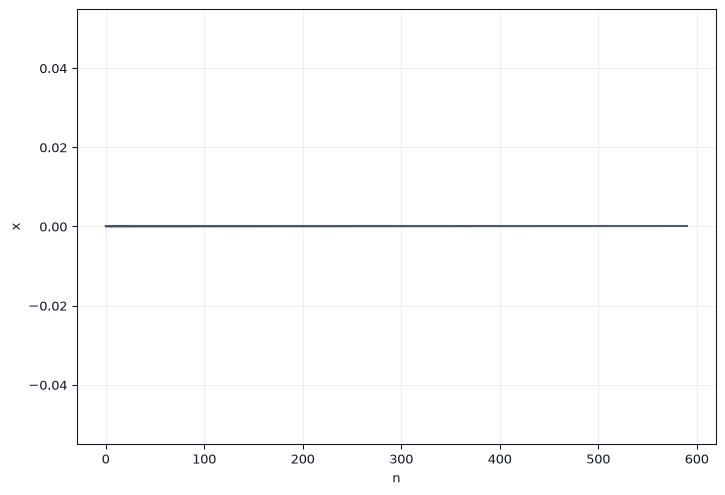
\includegraphics[width=0.72\textwidth,height=0.30\textheight,keepaspectratio]{../sprott/examples/thumbnails/synthetic_a_fixed_point_poor.png}
\caption{Control negativo \codigo{AMMM}: después del primer paso, la serie queda en
\(x_n=0\). La línea horizontal es el comportamiento esperado y permite interpretar
\codigo{fixed\_point} como colapso numérico de la cola, no como un fallo del dibujo.}
\label{fig:sprott-filtro-punto-fijo}
\end{figure}

\begin{figure}[H]
\centering
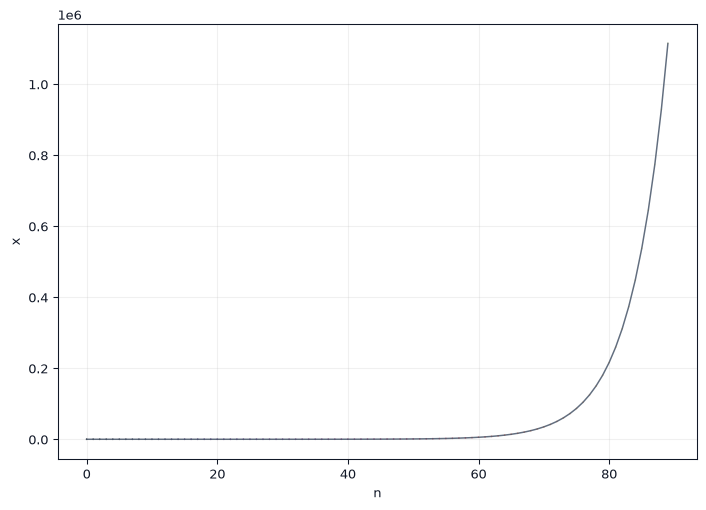
\includegraphics[width=0.72\textwidth,height=0.30\textheight,keepaspectratio]{../sprott/examples/thumbnails/synthetic_a_divergent_warning.png}
\caption{Control negativo \codigo{AMYM}: la escala vertical revela el crecimiento
geométrico hasta cruzar el umbral. Observe que \codigo{divergent} registra ese cruce
en una órbita finita; una ley asintótica de escape requiere una evaluación adicional.}
\label{fig:sprott-filtro-divergencia}
\end{figure}

Una consecuencia importante del orden de operaciones es que, si una simulación
en Python se trunca antes de alcanzar \(N_{\mathrm{tr}}\), la cola puede quedar
vacía y clasificarse como \codigo{unknown}, aun cuando el truncamiento ocurrió por
un cruce temprano. Antes de aceptar un resultado revise también la longitud de la
trayectoria completa, los valores no finitos y, si se usó el backend nativo, su
estado de salida.

\subsection{Cómo recorre códigos la búsqueda}

La búsqueda inicializa \(\operatorname{RNG}(\text{semilla})\) una sola vez. Si hay
un diccionario local \codigo{.DIC} cargado, ensaya primero las entradas visibles
desde la fila actual, continuando circularmente, hasta el máximo de intentos.
Cuando se agotan esas entradas genera códigos aleatorios de la familia elegida.
El valor predeterminado de la interfaz es 24 intentos. Cada código se simula,
descarta su transitorio y se clasifica antes de pasar al siguiente.

Los criterios visibles se interpretan actualmente así:
\[
\begin{array}{ll}
\text{\codigo{candidate\_chaotic}}&
   \text{acepta solamente ese estado},\\
\text{\codigo{acotado}}&
   \text{acepta todo estado distinto de \codigo{divergent}},\\
\text{\codigo{cualquier no divergente}}&
   \text{acepta todo estado distinto de \codigo{divergent}}.
\end{array}
\]
Por tanto, los dos últimos criterios son operativamente idénticos en esta versión
y ambos aceptan \codigo{unknown}. Además, el botón de búsqueda ejecuta el bucle de
forma síncrona y la pausa pertenece a otro contrato de ejecución. Una coincidencia de criterio es
una selección heurística, no una certificación de caos.

\subsection{Estimador rápido del máximo exponente de Lyapunov}

Para mapas y flujos polinomiales, el estimador de dos trayectorias parte de
\[
 \mathbf{x}_0=(0.1,\ldots,0.1),\qquad
 \mathbf{y}_0=\mathbf{x}_0+\varepsilon\mathbf{e}_1,\qquad
 \varepsilon=10^{-7}.
\]
Ambas trayectorias avanzan con el mismo paso numérico. Cada \(q=5\) pasos calcula
\[
 d_k=\|\mathbf{y}_k-\mathbf{x}_k\|_2,\qquad
 S\leftarrow S+\log\frac{d_k}{\varepsilon},
\]
y renormaliza
\[
 \mathbf{y}_k\leftarrow
 \mathbf{x}_k+\varepsilon
 \frac{\mathbf{y}_k-\mathbf{x}_k}{d_k}.
\]
Si \(m\) bloques completos fueron acumulados, devuelve
\[
 \widehat{\lambda}_{\max}=
 \frac{S}{m q\,\Delta t},\qquad
 \Delta t=
 \begin{cases}
 1,&\text{mapa},\\
 h,&\text{flujo}.
 \end{cases}
\]
Así, la unidad es por iteración para mapas y por unidad de tiempo para flujos.
Si la separación cae a \(10^{-300}\) o menos, devuelve
\(-\infty\) con estado de colapso. Si aparece un valor no finito o alguna de las
dos normas llega a \(10^6\), devuelve un valor no disponible.

\begin{idea}{Limitaciones exactas del Lyapunov rápido}
Este cálculo vuelve a comenzar desde \(\mathbf{x}_0\) y no elimina el transitorio
configurado en la simulación principal. En la tabla de intentos se ejecuta
solamente para estados \codigo{candidate\_chaotic} y usa 350 pasos, es decir,
70 renormalizaciones. Su umbral de divergencia es el valor propio \(10^6\), aunque
la simulación haya usado otro. Para familias especiales devuelve
\codigo{not\_available\_special\_family}, pues algunas dependen explícitamente de
\(n/N_{\max}\). Depende de horizonte, dirección inicial, \(h\), integrador y
precisión; un valor positivo finito apoya una hipótesis de sensibilidad, pero no
prueba caos ni una clasificación global de la dinámica.
\end{idea}

\section{Variables y proyecciones de las gráficas}

La visualización recibe primero los estados postransitorios finitos. Si exceden el
máximo de puntos, conserva índices aproximadamente equiespaciados entre el primero
y el último. El submuestreo sirve a la visualización; el análisis dinámico requiere
la trayectoria completa.

\begin{longtable}{p{0.25\linewidth} p{0.67\linewidth}}
\caption{Semántica de proyecciones, color y modos de dibujo.}\\
\toprule
Control & Cantidad representada\\
\midrule
\endfirsthead
\toprule
Control & Cantidad representada\\
\midrule
\endhead
\codigo{x-y}, \codigo{x-z}, \codigo{y-z},
\codigo{x-w}, \codigo{y-w}, \codigo{z-w} &
Dos componentes del estado en cada muestra. Una proyección puede ocultar cruces
o estructura presentes en otra coordenada.\\
\codigo{n-x}, \codigo{n-y}, \codigo{n-z} &
Índice local \(n=0,1,\ldots\) de la cola mostrada contra una componente. El índice absoluto anterior al transitorio y el tiempo físico de un flujo requieren sus convenciones de reconstrucción.\\
\codigo{3D x-y-z} &
Las tres primeras coordenadas. En dimensión 4, \(w\) queda oculto y puede
codificarse por color.\\
\codigo{esfera unitaria} &
Cada vector no nulo \((x,y,z)\) se divide entre su norma. Se conserva dirección y
se pierde radio; los vectores nulos se omiten. El color se calcula con el estado
original no normalizado.\\
\codigo{constante} &
Todos los puntos usan un solo color.\\
\codigo{tiempo} &
\(\operatorname{linspace}(0,1,N)\). Es progreso normalizado dentro de los puntos
mostrados, no tiempo físico ni la variable auxiliar \(w\).\\
\codigo{x}, \codigo{y}, \codigo{z}, \codigo{w} &
Valor de la coordenada elegida. Si se pide una coordenada ausente, la
implementación usa la última coordenada disponible; conviene no depender de ese
ajuste silencioso.\\
\codigo{radio} &
\(r_n=\|\mathbf{x}_n\|_2\), usando el conjunto completo de componentes del estado,
dos de la proyección.\\
\codigo{velocidad} &
\(\|\mathbf{x}_n-\mathbf{x}_{n-1}\|_2\), con cero en el primer punto. No divide
entre \(h\); en un flujo es desplazamiento por muestra, no velocidad física.\\
\codigo{bandas} &
Si el número de bandas es mayor que uno, normaliza el valor de color con su mínimo
y máximo finitos y asigna
\(\lfloor\operatorname{clip}(u,0,0.999999)B\rfloor\). Las bandas son una
cuantización cromática, no regiones invariantes.\\
\codigo{densidad} &
En 2D usa celdas hexagonales con tamaño de malla 170 y al menos un punto por
celda. En 3D el modo se dibuja como nube de puntos, no como estimación volumétrica
de densidad.\\
\bottomrule
\end{longtable}

\begin{figure}[H]
\centering
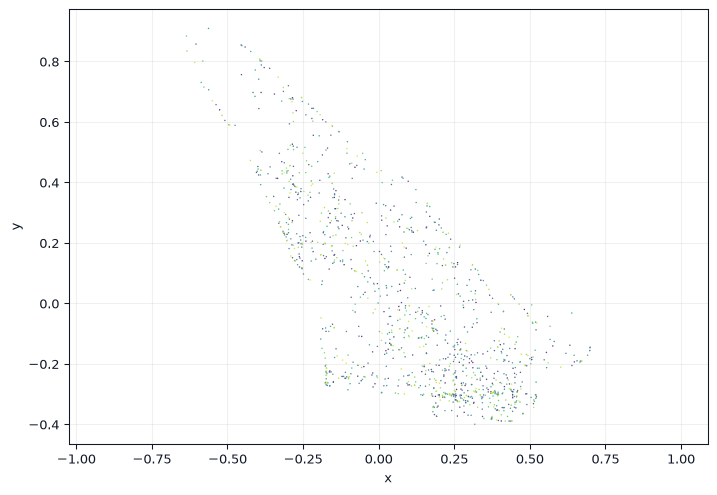
\includegraphics[width=0.73\textwidth,height=0.31\textheight,keepaspectratio]{../sprott/examples/thumbnails/synthetic_i_sparse_before_improvement.png}
\caption{Representación intencionalmente rala de una órbita tridimensional proyectada
en \(x\)-\(y\). Los huecos y la textura irregular invitan a aumentar el número de
muestras y reducir el tamaño de punto; interprételos con la malla y los criterios que distinguen vacíos invariantes y
con componentes desconectadas del sistema.}
\label{fig:sprott-muestreo-raleado}
\end{figure}

La igualdad de aspecto preserva escalas geométricas comparables en los dos ejes;
desactivarla puede estirar una estructura. El tamaño, alfa, fondo, paleta, líneas
y puntos afectan legibilidad, no las órbitas calculadas.\footnote{Lectura
complementaria: Sprott, \emph{Strange Attractors} (1993), cap.~4,
\emph{Attractors of Depth}: 4.1 \emph{Projections}, 4.2 \emph{Shadows},
4.3 \emph{Bands} y 4.4 \emph{Colors}; cap.~5, \emph{The Fourth Dimension},
en especial 5.2 \emph{Projections} y 5.3 \emph{Other Display Techniques}.}

\section{Los diecinueve flujos clásicos Sprott A--S}

Los nombres de esta sección pertenecen al catálogo de sistemas clásicos, no al
alfabeto de familias del código compacto. Todos son flujos autónomos
tridimensionales cuadráticos o de grado menor, sin parámetro ajustable en el
registro actual, y usan por omisión \((x_0,y_0,z_0)=(0.1,0.1,0.1)\).

Para graficarlos directamente abra la pestaña \control{Atractor 3D}, elija
\control{Sistema} \(\rightarrow\) \control{Sprott A}, \ldots,
\control{Sprott S}, integre y compare la vista 3D con \control{Retratos 2D}.
La última columna sugiere una primera proyección y se complementa con la inspección
de \(x\)-\(y\), \(x\)-\(z\) y \(y\)-\(z\). En el
\control{Explorador Sprott} también pueden codificarse como familia
\codigo{Q}, pues ésta representa flujos 3D cuadráticos; allí la \codigo{Q} es
una clase algebraica y no el nombre clásico Sprott Q.

{\small
\begin{longtable}{c p{0.58\linewidth} p{0.25\linewidth}}
\caption{Catálogo separado de los flujos clásicos Sprott A--S implementados.}\\
\toprule
Nombre & Ecuaciones & Cómo comenzar a graficarlo\\
\midrule
\endfirsthead
\toprule
Nombre & Ecuaciones & Cómo comenzar a graficarlo\\
\midrule
\endhead
Sprott A &
\(\dot x=y,\quad \dot y=-x+yz,\quad \dot z=1-y^2\). &
Selector \control{Sprott A}; 3D y \(x\)-\(y\).\\
Sprott B &
\(\dot x=yz,\quad \dot y=x-y,\quad \dot z=1-xy\). &
Selector \control{Sprott B}; 3D y \(x\)-\(z\).\\
Sprott C &
\(\dot x=yz,\quad \dot y=x-y,\quad \dot z=1-x^2\). &
Selector \control{Sprott C}; 3D y \(x\)-\(y\).\\
Sprott D &
\(\dot x=-y,\quad \dot y=x+z,\quad \dot z=xz+3y^2\). &
Selector \control{Sprott D}; 3D y \(x\)-\(z\).\\
Sprott E &
\(\dot x=yz,\quad \dot y=x^2-y,\quad \dot z=1-4x\). &
Selector \control{Sprott E}; 3D y \(x\)-\(y\).\\
Sprott F &
\(\dot x=y+z,\quad \dot y=-x+0.5y,\quad \dot z=x^2-z\). &
Selector \control{Sprott F}; 3D y \(x\)-\(z\).\\
Sprott G &
\(\dot x=0.4x+z,\quad \dot y=xz-y,\quad \dot z=-x+y\). &
Selector \control{Sprott G}; 3D y \(x\)-\(y\).\\
Sprott H &
\(\dot x=-y+z^2,\quad \dot y=x+0.5y,\quad \dot z=x-z\). &
Selector \control{Sprott H}; 3D y \(y\)-\(z\).\\
Sprott I &
\(\dot x=-0.2y,\quad \dot y=x+z,\quad \dot z=x+y^2-z\). &
Selector \control{Sprott I}; 3D y \(x\)-\(z\).\\
Sprott J &
\(\dot x=2z,\quad \dot y=-2y+z,\quad \dot z=-x+y+y^2\). &
Selector \control{Sprott J}; 3D y \(y\)-\(z\).\\
Sprott K &
\(\dot x=xy-z,\quad \dot y=x-y,\quad \dot z=x+0.3z\). &
Selector \control{Sprott K}; 3D y \(x\)-\(y\).\\
Sprott L &
\(\dot x=y+3.9z,\quad \dot y=0.9x^2-y,\quad \dot z=1-x\). &
Selector \control{Sprott L}; 3D y \(x\)-\(z\).\\
Sprott M &
\(\dot x=-z,\quad \dot y=-x^2-y,\quad \dot z=1.7+1.7x+y\). &
Selector \control{Sprott M}; 3D y \(x\)-\(y\).\\
Sprott N &
\(\dot x=-2y,\quad \dot y=x+z^2,\quad \dot z=1+y-2z\). &
Selector \control{Sprott N}; 3D y \(y\)-\(z\).\\
Sprott O &
\(\dot x=y,\quad \dot y=x-z,\quad \dot z=x+xz+2.7y\). &
Selector \control{Sprott O}; 3D y \(x\)-\(z\).\\
Sprott P &
\(\dot x=2.7y+z,\quad \dot y=-x+y^2,\quad \dot z=x+y\). &
Selector \control{Sprott P}; 3D y \(x\)-\(y\).\\
Sprott Q &
\(\dot x=-z,\quad \dot y=x-y,\quad
\dot z=3.1x+y^2+0.5z\). &
Selector \control{Sprott Q}; 3D y \(y\)-\(z\).\\
Sprott R &
\(\dot x=0.9-y,\quad \dot y=0.4+z,\quad \dot z=xy-z\). &
Selector \control{Sprott R}; 3D y \(x\)-\(y\).\\
Sprott S &
\(\dot x=-x-4y,\quad \dot y=x+z^2,\quad \dot z=1+x\). &
Selector \control{Sprott S}; 3D y \(x\)-\(z\).\\
\bottomrule
\end{longtable}
}

\begin{laboratorio}{El Sprott B clásico dentro de la familia Q}
Introduzca en el Explorador el código
\[
\codigolargo{QMMMMMMMMWMMWCMMMMMMMWMMMMCMMMM}.
\]
La familia \codigo{Q} usa la base
\[
\boldsymbol{\phi}_{3,2}
=(1,x,y,z,x^2,xy,xz,y^2,yz,z^2)^{\mathsf T}.
\]
Al separar los treinta coeficientes en tres filas de diez se recupera
\[
C=
\begin{pmatrix}
0&0&0&0&0&0&0&0&1&0\\
0&1&-1&0&0&0&0&0&0&0\\
1&0&0&0&0&-1&0&0&0&0
\end{pmatrix},
\]
es decir,
\[
\dot x=yz,\qquad \dot y=x-y,\qquad \dot z=1-xy,
\]
que coincide algebraicamente con el sistema clásico Sprott B de la tabla.

Use RK4, \(h=0.01\), \(N=30000\), transitorio \(4000\), umbral \(10^9\) y
\(\mathbf{x}_0=(0.1,0.1,0.1)\). Compare la figura con la obtenida mediante
\control{Atractor 3D} \(\rightarrow\) \control{Sprott B}. La coincidencia de
ecuaciones permite una verificación cruzada; las pequeñas diferencias numéricas
deben estudiarse controlando integrador, paso, número de muestras y transitorio.
\end{laboratorio}

\begin{figure}[H]
\centering
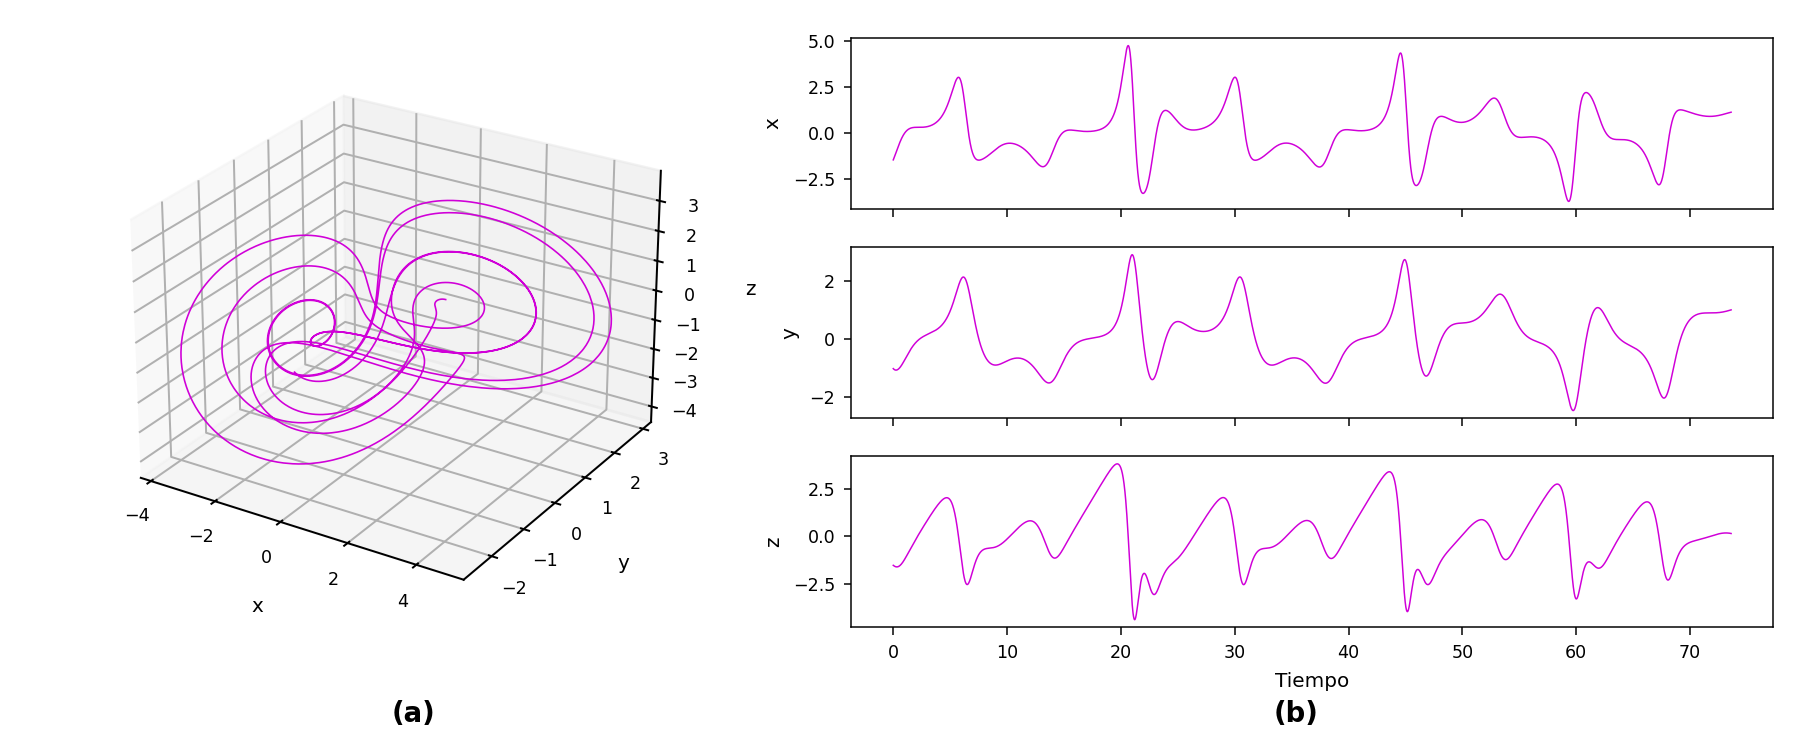
\includegraphics[width=0.97\textwidth,height=0.39\textheight,keepaspectratio]{../doc_figures/systems/sprott_b_phase_timeseries.png}
\caption{Lectura conjunta del sistema clásico Sprott B calculado con RK4. El panel
(a) resume la geometría espacial y el panel (b) conserva el orden temporal de
\(x(t)\), \(y(t)\) y \(z(t)\). Observe que los retornos entre regiones del retrato se
corresponden con excursiones de distinta amplitud en las tres componentes.}
\label{fig:sprott-b-fase-series}
\end{figure}

La conexión histórica y algebraica se desarrolla en estas lecturas.\footnote{Lectura
complementaria: Sprott, \emph{Elegant Chaos: Algebraically
Simple Chaotic Flows} (2010), cap.~3, \emph{Autonomous Dissipative Systems},
sección 3.4.2 \emph{Sprott Systems} y tabla 3.1. Para la transición de mapas a
campos continuos, véase también Sprott, \emph{Strange Attractors} (1993),
cap.~6, \emph{Fields and Flows}.}

\section{Prácticas con flujos, mapas y proyecciones 4D}

La tabla reúne valores de entrada completos. El estado esperado es el rótulo
heurístico del catálogo de ejemplos bajo esos parámetros; su interpretación se limita a
una propiedad demostrada para toda condición inicial o toda precisión numérica.

{\small
\setlength{\tabcolsep}{4pt}
\begin{longtable}{p{0.20\linewidth} p{0.18\linewidth} p{0.25\linewidth} p{0.19\linewidth}}
\caption{Ejemplos reproducibles incluidos en el Explorador.}\\
\toprule
Código & Sistema & Simulación & Visual inicial\\
\midrule
\endfirsthead
\toprule
Código & Sistema & Simulación & Visual inicial\\
\midrule
\endhead
\codigolargo{AWMA} &
Mapa 1D \(x^+=1-1.2x^2\). &
\(N=1400\), transitorio 80, umbral \(10^9\). Rótulo esperado:
\nolinkurl{periodic_or_low_complexity}. &
\codigo{n-x}; color \codigo{tiempo}; línea y puntos.\\
\codigolargo{EWMWAMMMPMMMM} &
Mapa 2D \(x^+=1+y-1.2x^2,\ y^+=0.3x\). &
\(N=28000\), transitorio 1200, umbral \(10^9\). Rótulo esperado:
\codigo{candidate\_chaotic}. &
\codigo{x-y}; puntos; color \codigo{tiempo}.\\
\codigolargo{QMMMMMMMMWMMWCMMMMMMMWMMMMCMMMM} &
Flujo 3D clásico Sprott B expresado en familia \codigo{Q}. &
RK4, \(h=0.01\), \(N=30000\), transitorio 4000, umbral \(10^9\).
Rótulo esperado: \codigo{candidate\_chaotic}. &
\codigo{3D x-y-z}; color \(z\); línea y puntos.\\
\codigolargo{MSLMFPHPIEFTPJJLOJNNTQQIINJUKJUUPPRMFIRIMELNKERJJIGJSGFLLOMSU} &
Mapa cuadrático 4D de catálogo sintético. &
\(N=52000\), transitorio 2600, umbral \(10^9\). Rótulo esperado:
\codigo{candidate\_chaotic}. &
\codigo{x-y}; color \(w\); puntos.\\
\codigolargo{AMMM} &
Mapa 1D \(x^+=0\). &
\(N=600\), transitorio 10, umbral \(10^9\). Rótulo esperado:
\codigo{fixed\_point}. &
\codigo{n-x}; ejes y retícula.\\
\codigolargo{AMYM} &
Mapa 1D \(x^+=1.2x\). &
\(N=420\), transitorio 0, umbral \(10^6\). Rótulo esperado:
\codigo{divergent}. &
\codigo{n-x}; ejes y retícula.\\
\bottomrule
\end{longtable}
}

\subsection{Código AWMA y trayectoria calculada}

La familia \codigo{A} usa \((1,x,x^2)\). Los caracteres
\codigo{WMA} dan \((1,0,-1.2)\), de modo que
\[
 x_{n+1}=1-1.2x_n^2,\qquad x_0=0.1.
\]
Los primeros valores son
\[
 x_1=0.988,\qquad
 x_2=-0.1713728,\qquad
 x_3\approx0.96476.
\]
La gráfica \codigo{n-x} permite observar el arranque y la repetición aproximada.
Después cambie el transitorio de 0 a 80 y confirme que lo descartado es el
segmento inicial, no una modificación de la recurrencia.

\begin{figure}[H]
\centering
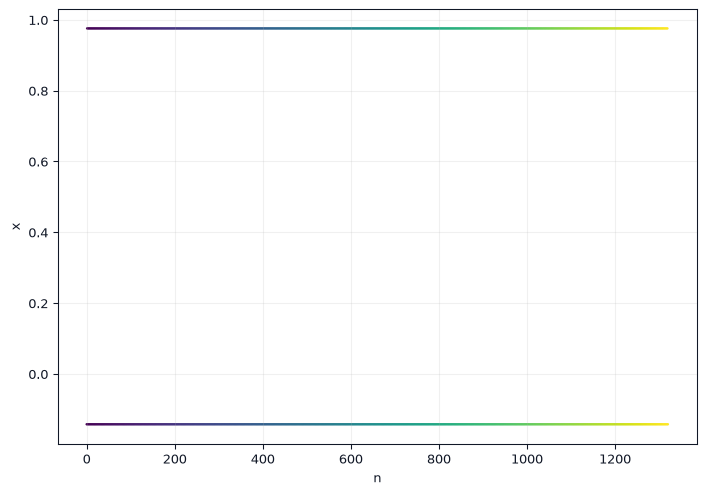
\includegraphics[width=0.72\textwidth,height=0.30\textheight,keepaspectratio]{../sprott/examples/thumbnails/synthetic_a_quadratic_time.png}
\caption{Serie reproducible del código \codigo{AWMA}. Lea primero el eje horizontal
como índice de iteración: las dos hileras de puntos revelan la alternancia asintótica
de período dos de una sola órbita. Cambiar el transitorio recorta su inicio, mientras
la recurrencia y sus valores posibles permanecen definidos por la misma regla cuadrática.}
\label{fig:sprott-awma-serie}
\end{figure}

\subsection{Códigos AMMM y AMYM para validación algebraica}

En \codigolargo{AMMM}, los tres coeficientes son cero:
\[
 x_1=0,\qquad x_n=0\quad(n\geq1).
\]
Una figura reducida a una línea o un punto es aquí el resultado matemático
correcto, no una falla del renderizador.

En \codigolargo{AMYM}, los coeficientes son \((0,1.2,0)\):
\[
 x_{n+1}=1.2x_n,\qquad x_n=0.1(1.2)^n.
\]
Con umbral \(10^6\), \(x_{88}\approx9.2886\times10^5\) y
\(x_{89}\approx1.1146\times10^6\). Por ello el cruce se predice antes de ejecutar
el programa. Este ejemplo separa una divergencia real de la regla iterada de una
inestabilidad creada por integrar un flujo con paso excesivo.

\subsection{Mapa 4D: ecuaciones y proyección}

Para
\[
\codigolargo{MSLMFPHPIEFTPJJLOJNNTQQIINJUKJUUPPRMFIRIMELNKERJJIGJSGFLLOMSU},
\]
la familia \codigo{M} usa los quince monomios cuadráticos 4D listados antes. Las
cuatro filas decodificadas son
\[
\begin{aligned}
\mathbf{c}_x={}&(0.6,-0.1,0,-0.7,0.3,-0.5,0.3,-0.4,\\
&\qquad -0.8,-0.7,0.7,0.3,-0.3,-0.3,-0.1),\\
\mathbf{c}_y={}&(0.2,-0.3,0.1,0.1,0.7,0.4,0.4,-0.4,\\
&\qquad -0.4,0.1,-0.3,0.8,-0.2,-0.3,0.8),\\
\mathbf{c}_z={}&(0.8,0.3,0.3,0.5,0,-0.7,-0.4,0.5,\\
&\qquad -0.4,0,-0.8,-0.1,0.1,-0.2,-0.8),\\
\mathbf{c}_w={}&(0.5,-0.3,-0.3,-0.4,-0.6,-0.3,0.6,-0.6,\\
&\qquad -0.7,-0.1,-0.1,0.2,0,0.6,0.8).
\end{aligned}
\]
Por tanto,
\[
 (x^+,y^+,z^+,w^+)^{\mathsf T}
 =C\,\boldsymbol{\phi}_{4,2}(x,y,z,w).
\]
Esta forma matricial es más verificable que copiar cuatro polinomios largos:
cada fila conserva exactamente el orden del código.

\begin{laboratorio}{Una órbita 4D requiere varias vistas}
Ejecute el código 4D con los parámetros de la tabla. Guarde primero \(x\)-\(y\)
con color por \(w\). Sin volver a simular, cambie a \(x\)-\(z\) con color por
\(y\), a \(z\)-\(w\) con color por radio y a esfera unitaria con color por \(w\).
Las cuatro imágenes provienen de los mismos datos y responden preguntas distintas.
Repita con la mitad de puntos visibles: la estructura gruesa debería persistir,
aunque cambien la densidad aparente y la saturación del color.
\end{laboratorio}

\begin{laboratorio}{Comparar RK4 y Euler sin confundir horizonte y paso}
Para el código del Sprott B clásico, conserve primero el experimento RK4 de la
tabla. Después use Euler con \(h=0.005\), \(N=16000\), transitorio 2000 y umbral
\(10^9\); grafique \(x\)-\(y\) con línea, ejes y retícula. Esta segunda corrida
es el ejemplo comparativo incluido en el catálogo. Como los horizontes y
transitorios físicos no coinciden con los de la corrida RK4, úsela para discutir
el aspecto visual del método, no como una prueba aislada de convergencia. Para una
comparación controlada, fije un mismo \(T\) y un mismo
\(T_{\mathrm{tr}}\), y ajuste \(N=T/h\).
\end{laboratorio}

\section{Archivos de exportación y datos de reproducción}

\subsection{Campos exportados en JSON y CSV}

El exportador JSON actual conserva el código, origen, archivo y línea de origen
cuando existen, parámetros de simulación
\((N,N_{\mathrm{tr}},h,\text{método},R_{\mathrm{div}})\), configuración visual,
clasificación, notas, fecha y advertencia de atribución. Es una base útil, pero no
incluye de forma automática:
\[
\begin{gathered}
\mathbf{x}_0,\quad \text{ecuaciones decodificadas},\quad
\text{backend efectivo y estado nativo},\quad
\text{vector de tiempos},\\
\text{rangos, medias y desviaciones},\quad
\widehat{\lambda}_{\max}\text{ y su estado},\quad
\text{semilla y máximo de intentos de una búsqueda}.
\end{gathered}
\]
Por ello, la reconstrucción completa de la procedencia computacional requiere
complementar el JSON con el registro de la simulación.

El CSV contiene solamente las filas finitas de la trayectoria postransitoria. Su
cabecera es \codigo{n,x,y,z,w} hasta la dimensión disponible y escribe cada
coordenada con 17 cifras significativas. La columna \codigo{n} se reinicia en cero
después del transitorio y después de eliminar filas no finitas. En un flujo no
exporta \(t\). Cuando la trayectoria conserva todas sus filas intermedias, puede reconstruirse
\[
 t_n=(n+N_{\mathrm{tr}})h;
\]
si hubo filtrado, esa fórmula ya no identifica de manera segura el índice
original. La imagen PNG, por su parte, registra el renderizado, no la trayectoria
completa.

\subsection{Registro manual de procedencia}

Para que otra persona pueda repetir una figura, adjunte al JSON y al CSV una ficha
con los siguientes campos:
\begin{enumerate}[label=\arabic*.]
 \item versión o identificador del software y sistema operativo;
 \item código limpio exacto, letra de familia, \(D\), \(O\), orden de monomios y
       ecuaciones o matriz \(C\);
 \item condición inicial completa;
 \item mapa o flujo; para flujo, integrador, \(h\), \(N\) y horizonte \(T\);
 \item transitorio en muestras y, para flujo, en tiempo físico;
 \item umbral de divergencia y backend efectivo;
 \item clasificación con sus tolerancias; estimación de Lyapunov con pasos,
       separación, intervalo de renormalización, estado y advertencias;
 \item semilla, máximo de intentos y procedencia \codigo{.DIC} o aleatoria si
       hubo búsqueda;
 \item proyección, color, bandas, máximo de puntos, modo de dibujo, paleta, alfa
       y resolución de exportación;
 \item comprobación de robustez pertinente: otro \(h\), otro integrador, más
       iteraciones, otro transitorio o condiciones iniciales cercanas.
\end{enumerate}

\begin{idea}{Tres niveles de afirmación}
Una cadena decodificada establece una ecuación. Una simulación reproducible
establece lo observado en una órbita finita y bajo una discretización concreta.
Una afirmación de caos, atractividad global o clasificación completa de cuencas
exige evidencia adicional. El Explorador ayuda con los dos primeros niveles y con
diagnósticos preliminares; el tercer nivel requiere su procedimiento de certificación.
\end{idea}

Para profundizar en búsqueda, registro y dimensión, continúe con estas
lecturas.\footnote{Lectura complementaria sobre búsqueda, registro y diccionarios:
Sprott, \emph{Strange Attractors} (1993), cap.~5, sección 5.6
\emph{Search and Destroy}, y apéndice F, \emph{Dictionaries}. Para sistemas de
mayor dimensión: Sprott, \emph{Elegant Chaos} (2010), cap.~6,
\emph{High-Dimensional Systems}.}
